\documentclass[xcolor=dvipsnames,aspectratio=169]{beamer}

% INCLUSIÓN DOS PAQUETES IMPRESCINDIBLES DE IDIOMA E CODIFICACIÓN DE CARACTERE.
\usepackage[T1]{fontenc}
\usepackage[english]{babel}
\usepackage[utf8]{inputenc}
\usepackage{csquotes}

%ACRONYMS para engadir un glosario de acronimos automatizado
% \usepackage[acronyms,nonumberlist,nopostdot,nomain,nogroupskip]{glossaries}
% \input{./acronyms.tex}

% PAQUETES PARA FIGURAS E GRAFICOS
\usepackage{graphicx}
%   \usepackage[pdftex]{graphicx}
  \usepackage{epstopdf}
   \graphicspath{{./img/}}
  % and their extensions so you won't have to specify these with
  % every instance of \includegraphics
   \DeclareGraphicsExtensions{.eps,.pdf,.png,.jpg}   
\usepackage{subfigure}
\usepackage{caption}
\usepackage[inkscapelatex=false]{svg}

%Tikz plots
\usepackage{tikz}
\usepackage{tikzscale}
\usetikzlibrary{plotmarks,patterns,decorations.pathreplacing,backgrounds,calc,arrows,arrows.meta,spy,matrix,backgrounds,shapes,math}

\tikzset{
    block/.style = {draw, rectangle, 
        minimum height=1cm, 
        minimum width=1.2cm, align=center},
    input/.style = {coordinate,node distance=1cm},
    output/.style = {coordinate,node distance=2cm},
    arrow/.style={draw, -latex,node distance=1.5cm},
    pinstyle/.style = {pin edge={latex-, black,node distance=1.5cm}},
    sum/.style = {draw, circle, node distance=1cm}
}

\newcommand{\tikzmark}[1]{\tikz[overlay,remember picture] \UE (#1) {};}
\newcommand{\DrawBox}[4][]{%
    \tikz[overlay,remember picture]{%
        \coordinate (TopLeft)     at ($(#2)+(-0.4em,1.6em)$);
        \coordinate (BottomRight) at ($(#3)+(0.4em,-1.0em)$);
        %
        \path (TopLeft); \pgfgetlastxy{\XCoord}{\IgnoreCoord};
        \path (BottomRight); \pgfgetlastxy{\IgnoreCoord}{\YCoord};
        \coordinate (LabelPoint) at ($(\XCoord,\YCoord)!0.5!(BottomRight)$);
        %
        \draw [red,#1] (TopLeft) rectangle (BottomRight);
        \UE [below, #1, fill=none, fill opacity=1] at (LabelPoint) {#4};
    }
}
\usepackage{pgfplots}
\pgfplotsset{compat=newest}
\pgfplotsset{plot coordinates/math parser=false}
\usepgfplotslibrary{patchplots,groupplots}

\tikzstyle{pinstyle} = [pin edge={to-,thin,black}]
\def\antenna{%
    -- +(0mm,4.0mm) -- +(2.625mm,7.5mm) -- +(-2.625mm,7.5mm) -- +(0mm,4.0mm) -- +(0mm,0mm)
}


% OUTROS PAQUETES DE USO COMUN. HOXE EN DIA OS COMPILADORES SON TAN RAPIDOS QUE EU METO TODOS SEMPRE
% \usepackage{float}
% \usepackage{ucs} 
% \usepackage{subcaption}
\usepackage{psfrag}
\usepackage{verbatim}
\usepackage{amsmath}
\usepackage{amsfonts} 
\usepackage{amssymb} 
\usepackage{amsthm}
\usepackage{pifont}
\usepackage{array}
\usepackage{listings}
\usepackage{stfloats}
\usepackage{algorithm} 
\usepackage{algorithmic} 
\usepackage{url} 
\usepackage{enumerate}
\usepackage{multirow}
\usepackage{wasysym}
\usepackage{cancel}
\usepackage{lmodern}


% DECLARACION DAS FONTES DA UVIGO
\usepackage[sfdefault]{roboto}
\usepackage{librebaskerville}
\setbeamerfont{title}{family=\librebaskerville,size=\Huge}
\setbeamerfont{subtitle}{family=\librebaskerville,size=\large}
% IMPORTANTE: a fonte 'campus' non queda ben para títulos de papers academicos,ç
% pero se de verdade se desexa empregar, seguir os seguintes pasos
% 1) Instalar o comando otftotfm en linux
% 2) sudo otftotfm -a -e texnansx campus_bold.otf CampusBold
% 3) asegurarse que o ficheiro auxiliar ./EETtemplateFiles/fonts/T1CampusBold.df está no directorio de traballo
% 4) descomentar a liña abaixo e comentar a liña que lle asigna librebaskerville arriba
\input{EETtemplateFiles/fonts/T1CampusBold.df}
\setbeamerfont{title}{family=\fontfamily{CampusBold},size=\Huge}

% DETLARACIÓN DO TEMA A USAR
% 
% ESTES TEMAS TEÑEN CABECEIRAS MOI GRANDES
% \usetheme{Berkeley} %large titlebar w/side dossier
% \usetheme{PaloAlto} 
% \usetheme{Copenhagen} %large titlebar w/2 side index
% \usetheme{Antibes} %large titlebar w/tree
% \usetheme{Singapore} %large titlebar w/balls evanescent
% \usetheme{Berlin} %large titlebar w/balls solid
% \usetheme{Dresden} %same as above with different color boxing
% \usetheme{Rochester} %large tittle-only titlebar
% ESTES TEMAS TEÑEN CABECEIRAS MEDIANAS
% \usetheme{CambridgeUS} %title titlebar w/current section
% \usetheme{Malmoe} %title titlebar w/current section Copenhagen style
% \usetheme{Madrid} %title titlebar w/page counter footer
% ESTES TEMAS TEÑEN CABECEIRAS DELGADAS
% \usetheme{Frankfurt} %small titlebar w/ progress balls
% \usetheme{metropolis} %metal
% ESTES TEMAS NON TEÑEN CABECEIRA DE COR, PERO SI TITULO SOBRE BRANCO
% \usetheme{Boadilla} %sombras e decoracion
\usetheme{Pittsburgh} %rectangulos planos
% ESTES TEMAS TEÑEN INDICES OU INFO NUNHA BARRA LATERAL GRANDE
% \usetheme{Goettingen} %right dossier evanescent
% \usetheme{Marburg} %right dossier fading to black
% \usetheme{Bergen} %notebook

%aspect modifiers
\useinnertheme{circles} %this makes item lists nicer
% \useoutertheme{infolines} %toggle thin info borders


% DECLARACIÓN DA COMBINACIÓN DE CORES A USAR. SE NON SE ESPECIFICA NADA TOMA A DEFINIDA POR DEFECTO
\definecolor{EETblue}{HTML}{0094e0} % a mate dark blue
\usecolortheme[named=EETblue]{structure} % EET UVigo blue
% outros temas de cores de beamer
% \usecolortheme{seagull} %makes title boxes gray color with blackr
% \usecolortheme{spruce} %makes title boxes pastel blue - gray color
% cores internos (items)
% \usecolortheme[named=Red]{structure} 
% \usecolortheme[named=Green]{structure} 
% \usecolortheme[named=OliveGreen]{structure} 
% \usecolortheme[named=PineGreen]{structure} 
% \usecolortheme[named=TealBlue]{structure} 
% \usecolortheme[named=SeaGreen]{structure}
% \usecolortheme[RGB={00,78,135}]{structure} % a dark cobalt blue 
% \usecolortheme[RGB={155,0,20}]{structure} % a slighlty darkened mate red

% MODIFICACIONS DAS CORES PARA A PAXINA DE TITULO SIMILAR Á OFICIAL
\setbeamercolor*{title}{use=structure,fg=structure.bg, bg=structure.fg}  
\setbeamercolor*{subtitle}{use=structure,fg=white}  
\setbeamercolor*{author}{use=structure,fg=structure.fg}
% \setbeamercolor*{institute}{use=structure,fg=structure.fg}
\setbeamercolor*{date}{use=structure,fg=structure.fg}
\setbeamertemplate{frametitle}[default][left]

% MODIFICACIONS DA SIDEBAR E FOOTLINE PARA INCLUIR AS IMAXES CORPORATIVAS.
\setbeamertemplate{footline}[text line]{%
  \parbox{\linewidth}{
    %ESTE TEXTO DA FOOTLINE PODESE MODIFICAR A GUSTO -----------------------------------------
    \insertshorttitle\hfill\insertshortauthor\hfill\insertpagenumber / \inserttotalframenumber
    %----------------------------------------------------------------------------------------
    \hfill
  
\includegraphics[width=.15\paperwidth,trim={0 2.5cm 3.5cm .75cm},clip]{EETtemplateFiles/img/Logotipo_ESCOLA.pdf}\vspace*{2pt}}}
\setbeamersize{sidebar width left = .10\paperwidth}
\setbeamertemplate{sidebar canvas left}{}
\setbeamertemplate{sidebar left}{%
  \vspace*{\fill}
  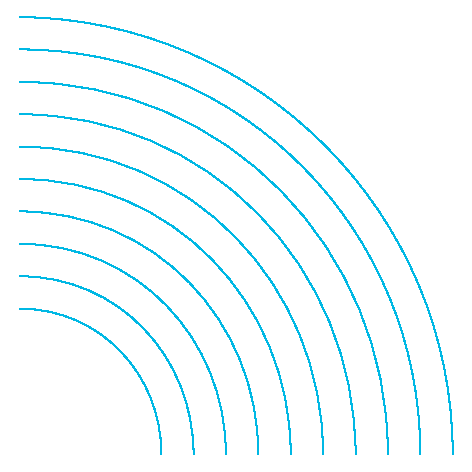
\includegraphics[width=.15\paperwidth,height=.15\paperwidth]{EETtemplateFiles/img/Simbolo_ESCOLA.pdf}\\
  
\includegraphics[width=.15\paperwidth,trim={.4cm .5cm .4cm 2.25cm},clip]{EETtemplateFiles/img/Logotipo_ESCOLA.pdf}
  \vspace*{-11pt}%
}

% MATH SYMBOLS

\newcommand{\field}[1]{\mathbb{#1}}

\DeclareMathOperator{\atan}{atan}
\DeclareMathOperator{\acos}{acos}
\DeclareMathOperator{\asin}{asin}

% \newcommand{\mb}[1]{\mathbf{#1}}


\newcommand{\A}{\mathbf{A}}
\newcommand{\B}{\mathbf{B}}
\newcommand{\Cb}{\mathbf{C}}
\newcommand{\D}{\mathbf{D}}
\newcommand{\Eb}{\mathbf{E}}
\newcommand{\F}{\mathbf{F}}
\newcommand{\Gb}{\mathbf{G}}
\newcommand{\Hb}{\mathbf{H}}
\newcommand{\I}{\mathbf{I}}
\newcommand{\J}{\mathbf{J}}
\newcommand{\Kb}{\mathbf{K}}
\newcommand{\Lb}{\mathbf{L}}
\newcommand{\M}{\mathbf{M}}
\newcommand{\N}{\mathbf{N}}
\newcommand{\Ob}{\mathbf{O}}
\newcommand{\Pb}{\mathbf{P}}
\newcommand{\Q}{\mathbf{Q}}
\newcommand{\R}{\mathbf{R}}
\newcommand{\Sb}{\mathbf{S}}
\newcommand{\T}{\mathbf{T}}
\newcommand{\U}{\mathbf{U}}
\newcommand{\V}{\mathbf{V}}
\newcommand{\W}{\mathbf{W}}
\newcommand{\X}{\mathbf{X}}
\newcommand{\Y}{\mathbf{Y}}
\newcommand{\Z}{\mathbf{Z}}
\newcommand{\Dl}{\mathbf{\boldsymbol{\Delta}}}
\newcommand{\Sg}{\mathbf{\boldsymbol{\Sigma}}}
\newcommand{\Ld}{\mathbf{\boldsymbol{\Lambda}}}
\newcommand{\Ph}{\mathbf{\boldsymbol{\Phi}}}
\newcommand{\Ps}{\mathbf{\boldsymbol{\Psi}}}
\newcommand{\Up}{\mathbf{\boldsymbol{\Upsilon}}}
\newcommand{\Xib}{\mathbf{\boldsymbol{\Xi}}}
% \newcommand{\D}{\mathbf{D}}
\newcommand{\one}{\mathbf{1}}
\newcommand{\zero}{\mathbf{0}}

\newcommand{\ab}{\mathbf{a}}
\newcommand{\bb}{\mathbf{b}}
\newcommand{\cc}{\mathbf{c}}
\newcommand{\dd}{\mathbf{d}}
\newcommand{\e}{\mathbf{e}}
\newcommand{\f}{\mathbf{f}}
\newcommand{\g}{\mathbf{g}}
\newcommand{\h}{\mathbf{h}}
\newcommand{\ib}{\mathbf{i}}
\newcommand{\jb}{\mathbf{j}}
\newcommand{\kb}{\mathbf{k}}
\newcommand{\lb}{\mathbf{\ell}}
\newcommand{\m}{\mathbf{m}}
\newcommand{\n}{\mathbf{n}}
\newcommand{\ob}{\mathbf{o}}
\newcommand{\pp}{\mathbf{p}}
\newcommand{\q}{\mathbf{q}}
\newcommand{\rr}{\mathbf{r}}
\newcommand{\s}{\mathbf{s}}
\newcommand{\uu}{\mathbf{u}}
\newcommand{\vv}{\mathbf{v}}
\newcommand{\w}{\mathbf{w}}
\newcommand{\x}{\mathbf{x}}
\newcommand{\y}{\mathbf{y}}
\newcommand{\z}{\mathbf{z}}
\newcommand{\al}{\mathbf{\boldsymbol{\alpha}}}
\newcommand{\vmu}{\mathbf{\boldsymbol{\mu}}}
\newcommand{\vlambda}{\mathbf{\boldsymbol{\lambda}}}
\newcommand{\vphi}{\mathbf{\boldsymbol{\phi}}}
\newcommand{\vpsi}{\mathbf{\boldsymbol{\psi}}}
\newcommand{\vrho}{\mathbf{\boldsymbol{\rho}}}
\newcommand{\vups}{\mathbf{\boldsymbol{\upsilon}}}
\newcommand{\vxi}{\mathbf{\boldsymbol{\xi}}}

\newcommand{\rank}{\textnormal{rank}}
% \newcommand{\trace}{\textnormal{trace}}
\newcommand{\exptr}{\textnormal{exptr}}
\newcommand{\tr}{\textnormal{tr}}
% \newcommand{\vstack}{\textnormal{vec}}
% \newcommand{\diag}{\textnormal{diag}}
\newcommand{\vstack}[1]{\Xib_{#1}}
\newcommand{\diag}[1]{\Ld_{#1}}
\newcommand{\tnsr}[2]{\underline{\mathsf{#1}}_{#2}}
\newcommand{\tmult}[1]{\underset{#1}{\times}}

\DeclareMathOperator{\Prob}{Prob}
%  |x>
\newcommand{\ket}[1]{\left\vert#1\right\rangle}
%  <x|
\newcommand{\bra}[1]{\left\langle#1\right\vert}
%  <x|y>
\newcommand{\braket}[2]{\left< #1 \vphantom{#2}\,
                        \right\vert\left.\!\vphantom{#1} #2 \right>}
%  <x|a|y>
\newcommand{\sandwich}[3]{\left< #1 \vphantom{#2 #3} \right|
                          #2 \min\left(\vphantom{#1 #2} #3 \right>}

\newcommand{\pd}[2]{\frac{\partial #1}{\partial #2}}
%  d/dt
\newcommand{\ddt}{\frac{d}{dt}}
%  D/Dx
\newcommand{\pdd}[1]{\frac{\partial}{\partial#1}}
%  |x|
\newcommand{\abs}[1]{\left\vert#1\right\vert}
%  k_{x}
\newcommand{\kv}[1]{\mathbf{k}_{#1}}
%  \textnormal{E}_{domain of integration}{variable}
\newcommand{\Ex}[2]{{\mathbb{E}_{#1}\left[#2\right]}}
\newcommand{\CEx}[3]{{\mathbb{E}_{#1}\left[#2|#3\right]}}
\newcommand{\CInf}[3]{{\textnormal{I}\left(#1;#2|#3\right)}}
\newcommand{\Inf}[2]{{\textnormal{I}\left(#1;#2\right)}}
\newcommand{\CEnt}[2]{{\textnormal{H}\left(#1|#2\right)}}
\newcommand{\Ent}[1]{{\textnormal{H}\left(#1\right)}}
\newcommand{\dCEnt}[2]{{\textnormal{h}\left(#1|#2\right)}}
\newcommand{\dEnt}[1]{{\textnormal{h}\left(#1\right)}}

\newcommand{\cmark}{\ding{51}}%
\newcommand{\xmark}{\ding{55}}%
\newcommand{\itempro}{\item[\textcolor{KYJade}{\Large \cmark}]}
\newcommand{\itemcontra}{\item[\textcolor{ARust}{\Large \xmark}]}
\newcommand\Tau{\mathcal{T}}
%Figure and format fixes


\renewcommand{\figurename}{Fig.}
\newcommand{\PESrule}{\noindent\rule{.57\columnwidth}{0.1mm}}

%theroem environments
% If using amsthm package, we need to delete these theorems before giving them our own definition. does not work for theorem
% \let\theorem\relax
\let\definition\relax
\let\lemma\relax
\let\corollary\relax
\let\example\relax
%
% \newtheorem{theorem}{Theorem}
\newtheorem{definition}{Definition}
\newtheorem{lemma}{Lemma}
\newtheorem{corollary}{Corollary}
\newtheorem{conjecture}{Conjecture}
\theoremstyle{plain}
\newtheorem{remark}{Remark}
\newtheorem{proposition}{Proposition}
\newtheorem{example}{Example}
\newtheorem{homework}{Homework}

%Colors
   \definecolor{blueH3}{rgb}{0,.5,1}
   \definecolor{blueH2}{rgb}{0,0.25,0.75}
   \definecolor{blueH1}{rgb}{0,0,0.5}   
   \definecolor{grayOldText}{rgb}{.5,.5,.5}
   \definecolor{VCobalt}{HTML}{005682}
   \definecolor{TZTeal}{HTML}{008080}
   \definecolor{TZTealfaded}{HTML}{F0FFFF}
   \definecolor{KYJade}{HTML}{008151}
   \definecolor{ARust}{HTML}{a10000}
   \definecolor{FFucsia}{HTML}{7000c3}   
   \definecolor{TAMustard}{HTML}{a1a100}
   \definecolor{Tangerine}{HTML}{d45500}
   
   
% Tikz 
% signal block diagram components
\tikzset{
    block/.style = {draw, rectangle, 
        minimum height=1cm, 
        minimum width=1.2cm, align=center},
    input/.style = {coordinate,node distance=1cm},
    output/.style = {coordinate,node distance=2cm},
    arrow/.style={draw, -latex,node distance=1.5cm},
    pinstyle/.style = {pin edge={latex-, black,node distance=1.5cm}},
    sum/.style = {draw, circle, node distance=1cm}
}
\tikzstyle{pinstyle} = [pin edge={to-,thin,black}]
\def\antenna{%
    -- +(0mm,4.0mm) -- +(2.625mm,7.5mm) -- +(-2.625mm,7.5mm) -- +(0mm,4.0mm) -- +(0mm,0mm)
}
% Overlay highlights on top of the page
\newcommand{\markOverlay}[1]{\tikz[overlay,remember picture] \node (#1) {};}
\newcommand{\drawOverlayBox}[4][]{%
    \tikz[overlay,remember picture]{%
        \coordinate (TopLeft)     at ($(#2)+(-0.4em,1.6em)$);
        \coordinate (BottomRight) at ($(#3)+(0.4em,-1.0em)$);
        %
        \path (TopLeft); \pgfgetlastxy{\XCoord}{\IgnoreCoord};
        \path (BottomRight); \pgfgetlastxy{\IgnoreCoord}{\YCoord};
        \coordinate (LabelPoint) at ($(\XCoord,\YCoord)!0.5!(BottomRight)$);
        %
        \draw [red,#1] (TopLeft) rectangle (BottomRight);
        \node [below, #1, fill=none, fill opacity=1] at (LabelPoint) {#4};
    }
}
\newcommand{\drawOverlayLine}[4][]{%
    \tikz[overlay,remember picture]{%
        \draw [red,#1] ($(#2)$) -- node{#4} ($(#3)$);
    }
}
\newcommand{\drawOverlayCircle}[4][]{%
    \tikz[overlay,remember picture]{%
        \draw [red,#1] ($(#2)$) circle (#3) node{#4};
    }
}
   
   %%%%%%%%%%%%%%%%%%%%%%%%%%%%%%%%%%%%%%%%%%%%%%%%%%%%%%%%%%%%%%%%%
%% The following definitions are to extend the LaTeX algorithmic 
%% package with SWITCH statements and one-line structures.
%% The extension is by 
%%   Prof. Farn Wang 
%%   Dept. of Electrical Engineering, 
%%   National Taiwan University. 
%% 
\newcommand{\SWITCH}[1]{\STATE \textbf{switch} (#1)}
\newcommand{\ENDSWITCH}{\STATE \textbf{end switch}}
\newcommand{\CASE}[1]{\STATE \textbf{case} #1\textbf{:} \begin{ALC@g}}
\newcommand{\ENDCASE}{\end{ALC@g}}
\newcommand{\CASELINE}[1]{\STATE \textbf{case} #1\textbf{:} }
\newcommand{\DEFAULT}{\STATE \textbf{default:} \begin{ALC@g}}
\newcommand{\ENDDEFAULT}{\end{ALC@g}}
\newcommand{\DEFAULTLINE}[1]{\STATE \textbf{default:} }
%% 
%% End of the LaTeX algorithmic package extension.

\newcounter{MYtempeqncnt}


%%%%%%%%%%%%%%%%%%%%%%%%%%%%%%%%%%%%%%%
% Commands to recall text later
%%%%%%%%%%%%%%%%%%%%%%%%%%%%%%%%%%%%%%%
\makeatletter
\newcommand\remembertext[2]{% #1 is a key, #2 is the text
  \immediate\write\@auxout{\unexpanded{\global\long\@namedef{mytext@#1}{#2}}}%
  #2%
}
%
\newcommand\recalltext[1]{%
  \ifcsname mytext@#1\endcsname
    \@nameuse{mytext@#1}%
  \else
    ``??''
  \fi
}

%%%%%%%%%%%%%%%%%%%%%%%%%%%%%%%%%%%%%%%%%%%%%%%%%%%%%%%%%%%%%%%%%%%%%%%%%%%%%%%%%%
%%% Paolo Casari: macros for automating section titling and comment formatting %%%
%%%%%%%%%%%%%%%%%%%%%%%%%%%%%%%%%%%%%%%%%%%%%%%%%%%%%%%%%%%%%%%%%%%%%%%%%%%%%%%%%%
\newcounter{myequationcnt}

\newcounter{rcnt}
\newcounter{ccnt}

\newcommand{\newreviewernopagebreak}[1]{\vspace{5em} \setcounter{ccnt}{0}\section*{\normalsize Comments of #1}\vspace{4mm}}

\newcommand{\ThisIsTheEditorNoPageBreak}{\setcounter{ccnt}{0}\section*{\Large Comments of the Editor}\vspace{3mm}}
\newcommand{\ThisIsTheEditor}{\clearpage \ThisIsTheEditorNoPageBreak}
\newcommand{\ThisIsANewReviewerNoPageBreak}[1]{\vspace{5em} \refstepcounter{rcnt}\label{r#1}\setcounter{ccnt}{0}\section*{\Large Comments of Reviewer \arabic{rcnt}}\vspace{3mm}}
\newcommand{\ThisIsANewReviewer}[1]{\clearpage\vspace{-5em} \ThisIsANewReviewerNoPageBreak{#1}}

\newcommand{\edcomment}[1]{
\begin{tcbremark}
\color{VCobalt}
    \refstepcounter{ccnt}\label{e\arabic{ccnt}}\noindent\textbf{\boldmath\emph{Comment E.\arabic{ccnt}:}} #1\vspace{0.2cm}
\end{tcbremark}
}
\newcommand{\refedcomment}[1]{E.\ref{e#1}}

\newcommand{\revcomment}[1]{
\begin{tcbremark}
\color{VCobalt}
\refstepcounter{ccnt}\label{r\arabic{rcnt}c\arabic{ccnt}}\noindent\textbf{\boldmath\emph{Comment \arabic{rcnt}.\arabic{ccnt}:}} #1\vspace{0.2cm}
\end{tcbremark}
}
\newcommand{\refrevcomment}[2]{\ref{r#1}.\ref{r#1c#2}}

% \newcommand{\ouranswer}[1]{\noindent\emph{Answer:} #1\vspace{0.6cm}}
% \newcommand{\citepap}[1]{\vspace{0.33cm}\begin{minipage}{0.05\textwidth} $\phantom{A}$  \end{minipage}\begin{minipage}{0.85\textwidth}\renewcommand{\baselinestretch}{1.15}\small \emph{#1} \end{minipage}\vspace{0.3cm}}

\newlength{\ansspace}
\addtolength{\ansspace}{0.6cm}
\newcommand{\ansbreak}{\vspace{\ansspace}}

\newlength{\stdleftskip}
\addtolength{\stdleftskip}{\leftskip}
\newlength{\stdrightskip}
\addtolength{\stdrightskip}{\rightskip}
\newlength{\citeskip}
\addtolength{\citeskip}{2em}
\newcommand{\oldbaselinestretch}{1.5}

\newcommand{\setcitepapskip}{%
    \leftskip\citeskip %
    \rightskip\citeskip %
    \renewcommand{\baselinestretch}{1.15}\small%
    \vspace{0.6em}%
    \noindent%
}

\newcommand{\resetLRmargins}{%
    \leftskip\stdleftskip %
    \rightskip\stdrightskip %
    \renewcommand{\baselinestretch}{\oldbaselinestretch}\normalsize %
    \vspace{0.6em}
}

\newcommand{\emans}{\emph{Answer:\ }}


%---------------
% LIMIAR
%---------------
%configuracion de opcions de beamer persoais, pero alleas ao estilo

% COMANDO QUE INTRODUCE UNHA DIAPOSITIVA CUN ÍNDICE NO QUE APARECEN VELADAS TÓDALAS SECCIÓNS MENOS A ACTUAL. ÚTIL PARA INTRODUCIR OS TÍPICOS ÍNDICES INTERMEDIOS.
\newcommand{\Inter}{\frame{\tableofcontents[currentsection]}}
\newcommand{\inter}{\frame{\tableofcontents[currentsection,currentsubsection]}}

% Pes de imaxe
\renewcommand{\figurename}{Fig.}
\addto\captionsenglish{\renewcommand{\figurename}{Fig.}}
\setbeamertemplate{caption}[numbered]

%ESTE PAQUETE PERMITE POÑER A BIBLIOGRAFIA AO PE DE PAXINA CON CONFIGURACIONS ESTETICAS PERSOAIS
% \usepackage[style=ieee,doi=false,isbn=false,url=true,backend=bibtex]{biblatex}
% \bibliography{./bibliografia.bib}
% \newrobustcmd*{\footfullcitenomark}{%
%   \AtNextCite{%
%     \let\thefootnote\relax 
%     \let\mkbibfootnote\mkbibfootnotetext
%     }%
%   \footfullcite}

%paquete para engadir notas de guion ao pdf
\usepackage{pgfpages}
% \setbeameroption{show only notes} 
% \setbeameroption{show notes}
% \setbeameroption{show notes on second screen=right}
% DATOS DO DOCUMENTO
\title[CDA]{Advanced Digital Communications}
\subtitle{Session 1: MIMO Communication Model}
\author[FGC]{\underline{Felipe G\'omez-Cuba}}
\institute[GPSC]{
\begin{columns}[T]
\begin{column}{5cm}\centering
Office A-204\\
Monday-Thursday 15:00-16:30\\
\texttt{gomezcuba@gts.uvigo.es}\\
\end{column}
\end{columns}
}

\date{}

\begin{document}

% Diapositiva co título
\frame[plain]{\titlepage}
% 
% \frame{\tableofcontents}
% \note[itemize]{
% \item First we will look at what the receiver needs from the CSI
% \item Second we will look at several ML estimators for vector under known linear expressions
% \item Finally we will look at delay-support CS estimators for $P_{\tau}$
% }

% \section{Sparse Wideband OFDM Channel}
% \subsection{Wideband Sparse Channel}
\section{Introduction}
\frame[allowframebreaks]{\frametitle{Why MIMO?}

\begin{figure}
 \centering
 \caption{Cellular subscribers and traffic growth}
 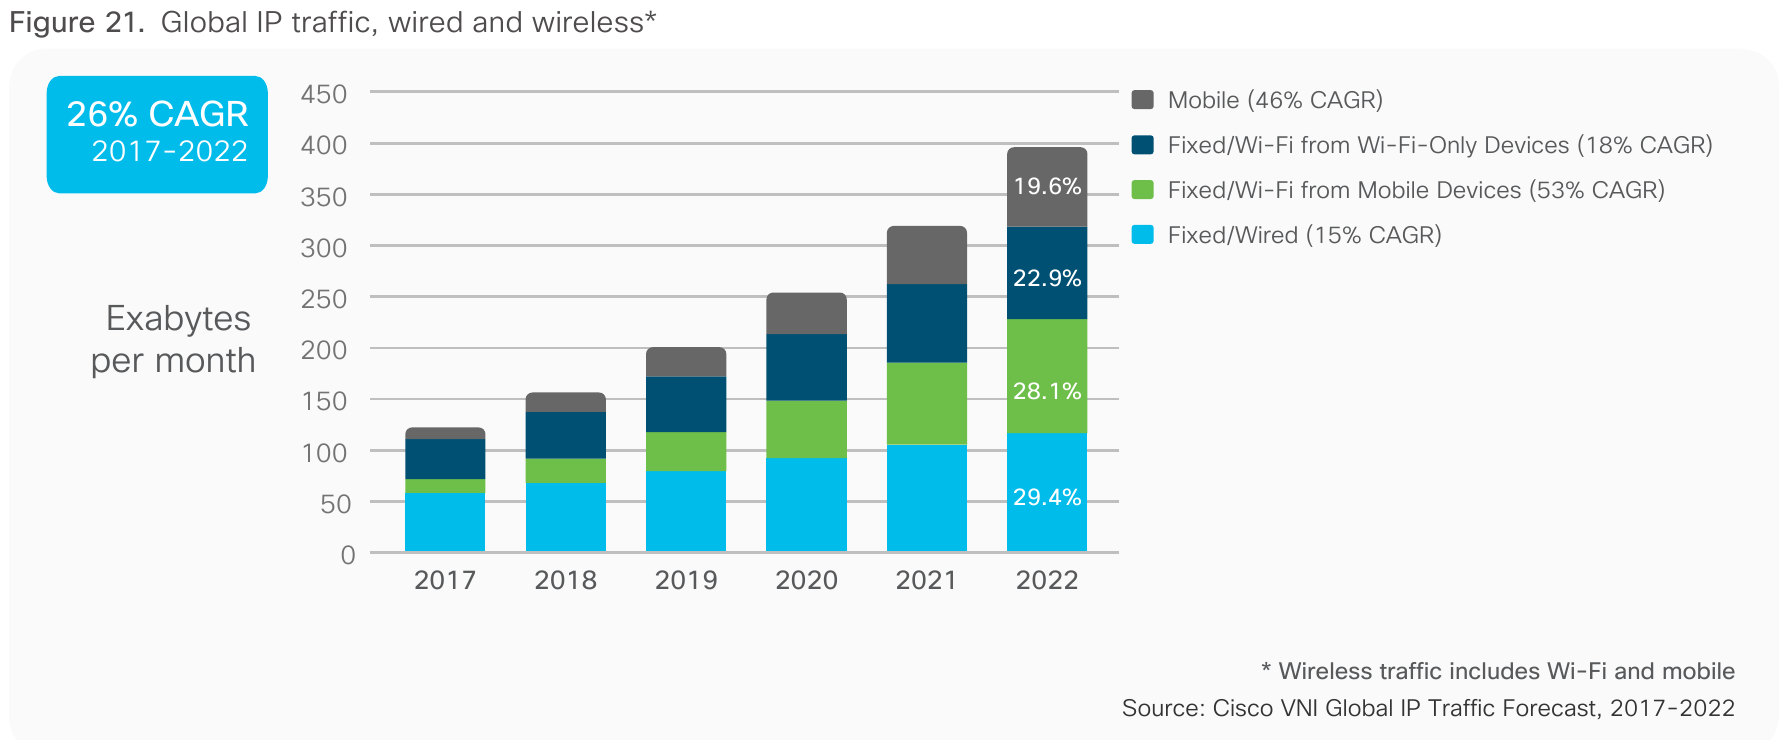
\includegraphics[width=.9\columnwidth]{traffic}
\end{figure}

\begin{figure}
 \centering
 \caption{Generations of 3GPP Standards}
 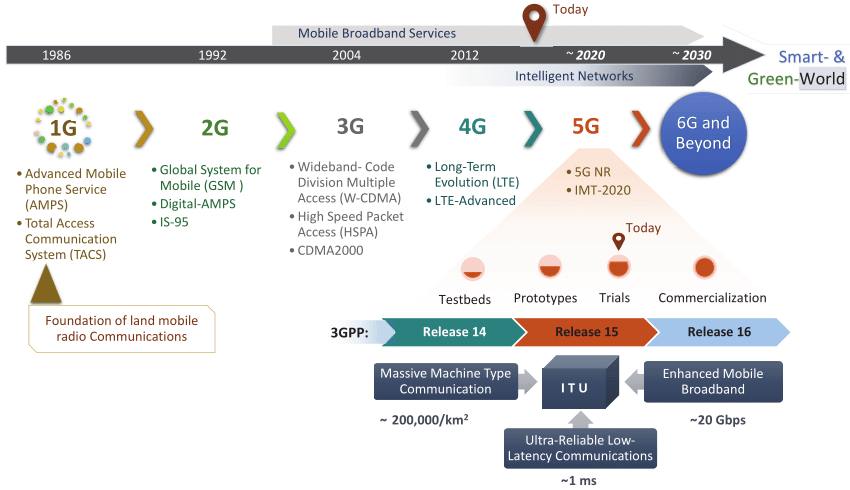
\includegraphics[width=.8\columnwidth]{generations}
\end{figure}
\framebreak
How to increase cellular system capacity
\begin{itemize}
 \item Tx. Power: increases interference
 \item Symbol Rate: spectrum is incredibly expensive, ADC difficult
 \item Density: cell size $<100$ m difficult
 \item \textbf{Number of antennas}:
\end{itemize}
\begin{figure}
 \centering
 \subfigure[1 antenna]{
    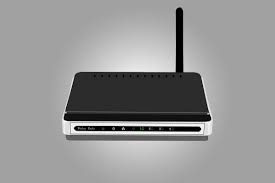
\includegraphics[width=.16\textwidth]{1antrouter}
 }
 \hspace{.1in}
 \subfigure[2 antennas]{
    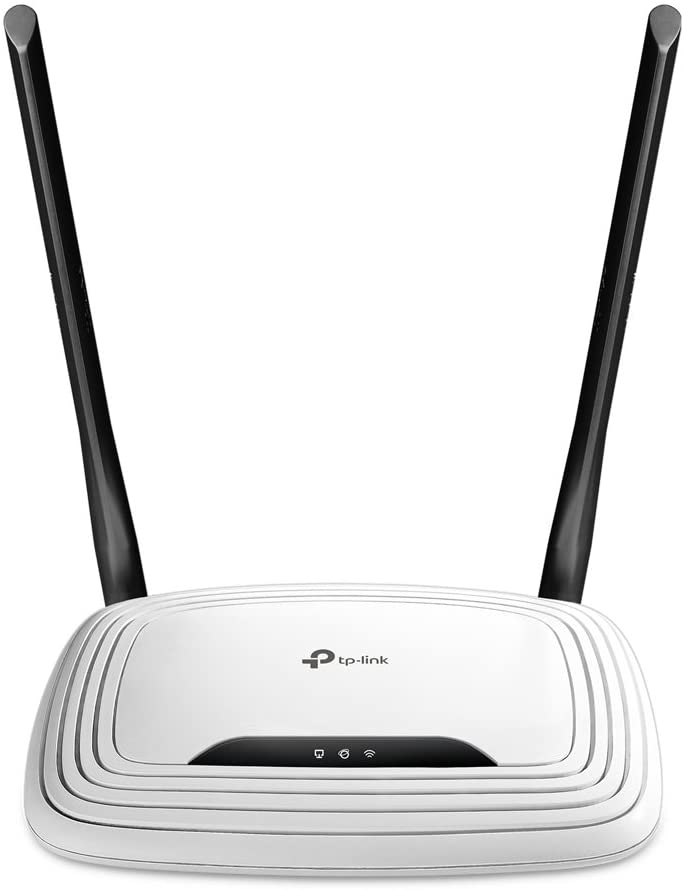
\includegraphics[width=.16\textwidth,trim={0 0 0 10cm},clip]{2antrouter}
 }
 \hspace{.1in}
 \subfigure[4 antennas]{
    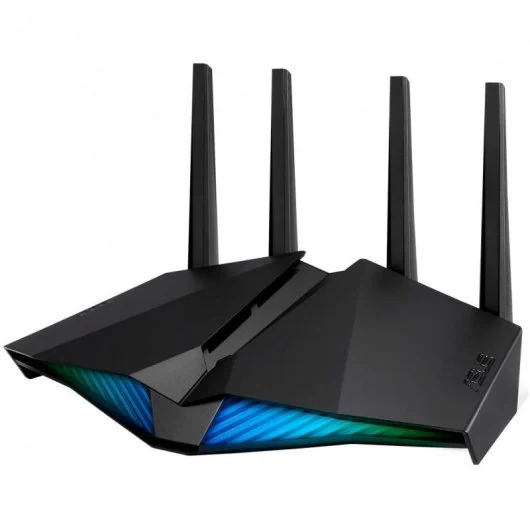
\includegraphics[width=.16\textwidth]{4antrouter}
 }
 \hspace{.1in}
 \subfigure[8 antennas]{
    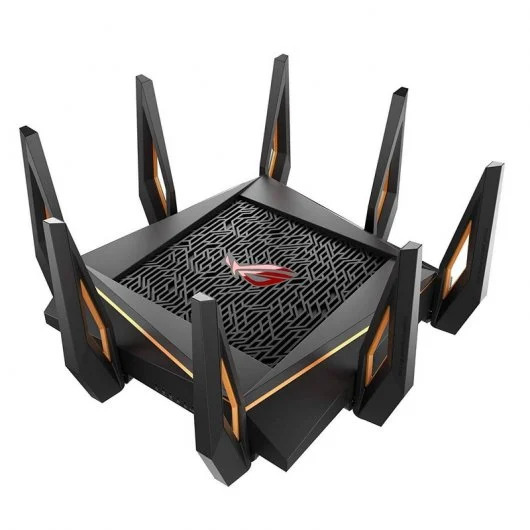
\includegraphics[width=.16\textwidth]{8antrouter}
 }
 \caption{Some WiFi Routers}
\end{figure}
}

\frame[allowframebreaks]{\frametitle{Classification of Wireless interfaces}
\begin{figure}
 \centering
 \caption{Single Input Single Output (SISO)}
 \includesvg[width=.7\columnwidth]{siso}
\end{figure}
\begin{figure}
 \centering
 \caption{Multiple Input Single Output (MISO)}
 \includesvg[width=.7\columnwidth]{miso}
\end{figure}
\begin{figure}
 \centering
 \caption{Single Input Multiple Output (SIMO)}
 \includesvg[width=.7\columnwidth]{simo}
\end{figure}
\begin{figure}
 \centering
 \caption{Multiple Input Multiple Output (MIMO)}
 \includesvg[width=.7\columnwidth]{mimo}
\end{figure}
}

\frame{\frametitle{Multipath Channel}
\begin{columns}
\begin{column}{8cm}
\begin{figure}
 \centering
 \caption{Multipath Channel}
 \includesvg[width=.9\columnwidth]{multipath}
\end{figure}
\vspace{.1in}
\end{column}
\begin{column}{4cm}
\begin{itemize}
 \item System of Linear Equations
    $$\begin{array}{c}y_1=h_{1,1}x_1+h_{1,2}x_2\\y_2=h_{2,1}x_1+h_{2,2}x_2\end{array}$$    
 \item Has solution if $h_{1,1},h_{1,2},h_{2,1},h_{2,2}$ are all different
\end{itemize}
\end{column}
\end{columns}

Paradigm shift in interpretation of multipath channel
\begin{itemize}
 \item Before: ``multipath is a problem, creates Inter-Symbol Interference''
 \item Now: ``multipath is an opportunity, creates degrees of freedom''
\end{itemize}
}

\section{Deterministic Channel Modeling}

\frame[allowframebreaks]{\frametitle{Discrete Equivalent Channel}
\begin{figure}
 \centering
 \caption{Digital Transmitter Block Diagram}
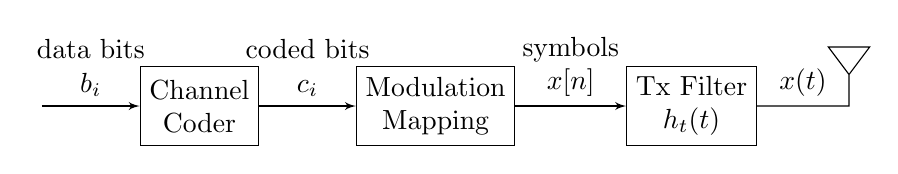
\begin{tikzpicture}[auto, node distance=2cm,>=latex']
    \node [input, name=input] {};
    \node [block, right of=input] (cc) {Channel\\ Coder};
    \draw [draw,->,align=center] (input) -- node {data bits\\ $b_i$} (cc);
    \node [block, right of=cc, node distance=3.cm] (mod) {Modulation\\ Mapping};
    \draw [->,align=center] (cc) -- node[name=c] {coded bits\\ $c_i$} (mod);
    \node [block, right of=mod, node distance=3.25cm] (txf) {Tx Filter\\ $h_t(t)$};
    \draw [->,align=center] (mod) -- node[name=s] {symbols\\$x[n]$} (txf);
    \node [output, right of=txf, node distance=2cm] (output) {};
    \draw [-] (txf) -- node[name=xt] {$x(t)$} (output) \antenna;            
\end{tikzpicture}
\end{figure}
\begin{itemize}
 \item CC maps data bits $b_i$ to coded bits $c_i$
 \item MM maps bits to symbols $x[n]\in \mathcal{C}$ (QAM, BPSK, PSK, etc.)
 \item TF maps discrete-time sequence $x[n]$ in continuous time signal
 $$x(t)=\sum_{n}x[n]h_t(t-nT)$$
\end{itemize}

\begin{figure}
 \centering
 \caption{Digital Receiver Block Diagram}
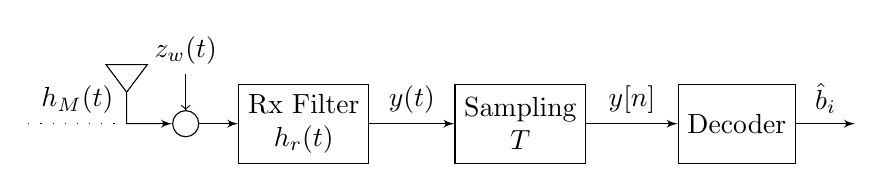
\begin{tikzpicture}[auto, node distance=2cm,>=latex']
    \node [input, name=channel] {};
    \node [input, name=input,right of=channel, node distance=1.25cm] {};
    \draw [draw,loosely dotted,-,align=center] (channel) -- node {$h_M(t)$} (input) ;
    \node [sum, right of=input, node distance=.75cm, pin={[pinstyle]above:$z_w(t)$}] (sum) {};
    \draw [draw,->,align=center] (input) \antenna -- (sum)  ;
    \node [block, right of=sum, node distance=1.5cm] (rxf) {Rx Filter\\ $h_r(t)$};
    \draw [draw,->,align=center] (sum) -- (rxf);
    \node [block, right of=rxf, node distance=2.75cm] (smp) {Sampling\\ $T$};
    \draw [->,align=center] (rxf) -- node[name=s] {$y(t)$} (smp);
    \node [block, right of=smp, node distance=2.75cm] (rec) {Decoder};
    \draw [->,align=center] (smp) -- node[name=s] {$y[n]$} (rec);
    \node [output, right of=rec, node distance=1.5cm] (output) {};
    \draw [->,align=center] (rec) -- node[name=s] {$\hat{b}_i$} (output); 
\end{tikzpicture}
\end{figure}
\begin{itemize}
\item AWGN Power Spectral Density $|Z_w(\omega)|^2=N_o$Watt/Hz\\
\item Colored noise $z(t)=z_w(t)*h_r(t)$
$$|Z(\omega)|^2=N_o|H_r(\omega)|^2$$
\item Continuous Equivalent Channel $h(t)=h_t(t)*h_M(t)*h_r(t)$
$$y(t)=\sum_n x[n]h(t-nT)+z(t)$$
\end{itemize}

\begin{itemize}
 \item Sample $y(t)$ with period $T_s$  
    $$y[n]=\sum_k x[k]h[n-k]+z[n]$$
 \item Equiv. to sampling $h(t)$ w.r.t. $\sum_n x[n]h(t-nT_s)$\\ \ \\
    
 \item If $h_r(t)$ satisfyies Nyquist zero-ISI criterion,
        $$\frac{1}{T_s}\sum_{k}\left|H_r(\frac{\omega-2\pi k}{T_s})\right|^2=1$$
        then $z[n]$ is white.\\ \ \\
\end{itemize}
 }
 
\frame[allowframebreaks]{\frametitle{Non-Dispersive SISO DEC}

\begin{figure}
 \centering
 \caption{Non-Dispersive Channel}
 \includesvg[width=.5\columnwidth]{nondispersive}
 \end{figure}
 \begin{itemize}
 \item Weak tails outside $t\in[0,T_s]$
    $$|h(t)|^2\simeq 0 \;\forall t\notin[0,T_s]$$
 \item Sampled is almost a delta
    $$h[n]\simeq h_0\delta[n]$$
 \end{itemize}
 
\framebreak
 \begin{itemize}
 \item There is no ISI in the Non-Dispervive DEC $$y[n]\simeq  h_0 x[n]+ z[n]$$\\ \ \\
 \item Signal To Noise Ratio
 \begin{itemize}
  \item $\Ex{}{|z[n]|^2} = \sigma_{z}^2 = N_oB$
  \item $\Ex{}{| h_0 x[n]|^2} = P|h_0|^2$
   $$\textnormal{SNR} = \frac{P|h_0|^2}{\sigma_{z}^2}$$\\ \ \\
 \end{itemize}
 \end{itemize}

\begin{figure}
 \centering
 \caption{Frequency Selective Channel (Dispersive)}
 \includesvg[width=.4\columnwidth]{dispersive}
 \end{figure}
 \begin{itemize}
\item For dispersive channels we can use OFDM
 \begin{itemize}
 \item CP length $M$, where $h(t)$ is ``contained'' in  $t\in[0,T_sM]$  
 \item $K\geq M $, each subcarrier experiences a Non-dispersive channel
    $$y[k]\simeq  h_0[k] x[k]+ z[k]$$
 \item SNR$[k]=\frac{\Ex{}{|x[k]|^2}|h_0[k]|^2}{\Ex{}{|z[k]|^2}}=\frac{\frac{P}{K}|h_0[k]|^2}{N_o\Delta f}=\frac{P|h_0[k]|^2}{N_o K\Delta f}=\frac{P|h_0[k]|^2}{N_o B}$
 \item $h_0[k]\simeq \texttt{FFT}(\{h(mT)\}_{m=0}^{M},K)$
 \end{itemize}
 \end{itemize}
}
 
\frame{\frametitle{Non-Dispersive SIMO DEC}
\begin{columns}
 \begin{column}{6cm}
    
\begin{figure}
 \centering
 \caption{SIMO Channel}
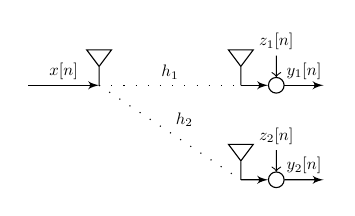
\begin{tikzpicture}[auto, node distance=2cm,>=latex', scale=0.6, every node/.style={scale=0.6}]
    \node [input, name=input] {};
    \node [input, right of=input, node distance=1.5cm, name=txant] {};
    \draw [draw] (txant) \antenna;
    \draw [draw,->,align=center] (input) -- node {$x[n]$} (txant);
    \node [input, right of=txant, node distance=3cm, name=rxant1] {};
    \node [input, below of=rxant1, node distance=2cm, name=rxant2] {};
    \draw [draw,loosely dotted,-,align=center] (txant)  -- node {$h_1$} (rxant1);
    \draw [draw,loosely dotted,-,align=center] (txant)  -- node {$h_2$} (rxant2);
    \draw [draw] (rxant1) \antenna;
    \draw [draw] (rxant2) \antenna;
    \node [sum, right of=rxant1, node distance=.75cm, pin={[pinstyle]above:$z_1[n]$}] (sum1) {};
    \node [sum, right of=rxant2, node distance=.75cm, pin={[pinstyle]above:$z_2[n]$}] (sum2) {};
    \draw [draw,->,align=center] (rxant1) -- (sum1);
    \draw [draw,->,align=center] (rxant2) -- (sum2);
    \node [input, right of=sum1, name=output1] {};
    \node [input, right of=sum2, name=output2] {};
    \draw [draw,->,align=center] (sum1) -- node {$y_1[n]$} (output1);
    \draw [draw,->,align=center] (sum2) -- node {$y_2[n]$} (output2);         
\end{tikzpicture}
\end{figure}
\begin{itemize}
\item Vector Notation
$$\y[n]=\h x[n] +\z[n]$$\\ \ \\
\end{itemize}
 \end{column}
 \begin{column}{6cm}
\begin{figure}
 \centering
 \caption{MISO Channel}
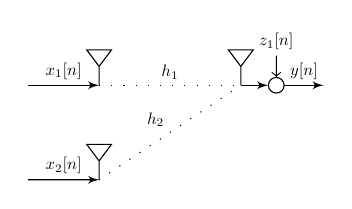
\begin{tikzpicture}[auto, node distance=2cm,>=latex', scale=0.6, every node/.style={scale=0.6}]
    \node [input, name=input1] {};
    \node [input, below of=input1, node distance=2cm, name=input2] {};
    \node [input, right of=input1, node distance=1.5cm, name=txant1] {};
    \node [input, right of=input2, node distance=1.5cm, name=txant2] {};
    \draw [draw] (txant1) \antenna;
    \draw [draw] (txant2) \antenna;
    \draw [draw,->,align=center] (input1) -- node {$x_1[n]$} (txant1);
    \draw [draw,->,align=center] (input2) -- node {$x_2[n]$} (txant2);
    \node [input, right of=txant1, node distance=3cm, name=rxant1] {};
    \draw [draw,loosely dotted,-,align=center] (txant1)  -- node {$h_1$} (rxant1);
    \draw [draw,loosely dotted,-,align=center] (txant2)  -- node {$h_2$} (rxant1);
    \draw [draw] (rxant1) \antenna;
    \node [sum, right of=rxant1, node distance=.75cm, pin={[pinstyle]above:$z_1[n]$}] (sum1) {};
    \draw [draw,->,align=center] (rxant1) -- (sum1);
    \node [input, right of=sum1, name=output1] {};
    \draw [draw,->,align=center] (sum1) -- node {$y[n]$} (output1);         
\end{tikzpicture}
\end{figure}
\begin{itemize}
\item Vector Notation
$$y[n]=\h^H \x[n] +z[n]$$\\ \ \\
\end{itemize}
 \end{column}
\end{columns}

% where 
$\y[n]=\left[\begin{array}{c}
 y_1[n]\\
 \vdots\\
 y_{n_r}[n]
\end{array}\right],\;
\h=\left[\begin{array}{c}
 h_1\\
 \vdots\\
 h_{n_r}
\end{array}\right]
,\;
\x[n]=\left[\begin{array}{c}
 x_1[n]\\
 \vdots\\
 x_{n_t}[n]
\end{array}\right]
 ,\;
\z[n]
=\left[\begin{array}{c}
 z_1[n]\\
 \vdots\\
 r_{n_r}[n]
\end{array}\right]
$
}
 
\frame{\frametitle{Non-Dispersive MIMO DEC}
\begin{figure}
 \centering
 \caption{MIMO Channel}
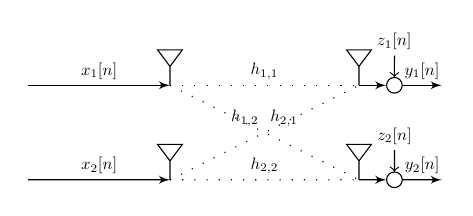
\begin{tikzpicture}[auto, node distance=2cm,>=latex', scale=0.6, every node/.style={scale=0.6}]
    \node [input, name=input1] {};
    \node [input, right of=input1, node distance=3cm, name=txant1] {};
    \draw [draw] (txant1) \antenna;
    \node [input, below of=input1, node distance=2cm,name=input2] {};
    \node [input, right of=input2, node distance=3cm, name=txant2] {};
    \draw [draw] (txant2) \antenna;
    \draw [draw,->,align=center] (input1) -- node {$x_1[n]$} (txant1);
    \draw [draw,->,align=center] (input2) -- node {$x_2[n]$} (txant2);
    \node [input, right of=txant1, node distance=4cm, name=rxant1] {};
    \node [input, below of=rxant1, node distance=2cm, name=rxant2] {};
    \draw [draw,loosely dotted,-,align=center] (txant1)  -- node {$h_{1,1}$} (rxant1);
    \draw [draw,loosely dotted,-,align=center] (txant1)  -- node {$h_{2,1}$} (rxant2);
    \draw [draw,loosely dotted,-,align=center] (txant2)  -- node {$h_{1,2}$} (rxant1);
    \draw [draw,loosely dotted,-,align=center] (txant2)  -- node {$h_{2,2}$} (rxant2);
    \draw [draw] (rxant1) \antenna;
    \draw [draw] (rxant2) \antenna;
    \node [sum, right of=rxant1, node distance=.75cm, pin={[pinstyle]above:$z_1[n]$}] (sum1) {};
    \node [sum, right of=rxant2, node distance=.75cm, pin={[pinstyle]above:$z_2[n]$}] (sum2) {};
    \draw [draw,->,align=center] (rxant1) -- (sum1);
    \draw [draw,->,align=center] (rxant2) -- (sum2);
    \node [input, right of=sum1, name=output1] {};
    \node [input, right of=sum2, name=output2] {};
    \draw [draw,->,align=center] (sum1) -- node {$y_1[n]$} (output1);
    \draw [draw,->,align=center] (sum2) -- node {$y_2[n]$} (output2);         
\end{tikzpicture}
\end{figure}
\begin{itemize}
\item $n_t\times n_r$ MIMO DEC Matrix Notation
$$\y[n]=\Hb \x[n] +\z[n]$$
where $
\Hb=\left[\begin{array}{cccc}
 h_{1,1}&\dots&h_{1,n_t}\\
 \vdots&\ddots&\vdots\\
 h_{n_r,1}&\dots&h_{n_r,n_t}\\
\end{array}\right]
$
\item Sometimes we can omit [n] for clarity $\y=\Hb \x +\z$
\end{itemize}
}

\frame[allowframebreaks]{\frametitle{Multi-dimensional Random Channel}
 \begin{itemize}
    \item Noise $\z$ Statistical Distribution
    \begin{itemize}
        \item Zero Mean $\Ex{}{z_{j}}=0  \;\Rightarrow\; \Ex{}{\z}=\zero$\\ \ \\
        \item Covariance Matrix 
        $$\K_{\z}=\Ex{}{\z \z^H}=\Ex{}{\left( \begin{array}{cccc}
                                                |z_1|^2&z_1z_2^*&\dots &z_1z_{n_r}^*\\
                                                z_2z_1^*&|z_2|^2&\dots &z_2z_{n_r}^*\\
                                               \vdots&\vdots&\ddots &\vdots\\
                                                z_{n_r}z_1^*&z_{n_r}z_2^*&\dots &|z_{n_r}|^2\\
                                               \end{array} \right)}$$
        \item Spatially Uncorrelated i.d. Noise $\Ex{}{z_2z_1^*}=0\Rightarrow \K_{\z}=\sigma_z^2\I$
        \item Total received noise power 
        $$\Ex{}{\|\z\|^2}=\Ex{}{\z^H\z}=\sum_{j=1}^{n_r} \Ex{}{|z_j|^2}=\tr\{\K_{\z}\}\stackrel{i.i.d.}{=}n_r\sigma_z^2$$
    \end{itemize}
    \item Input $\x$ Statistical Distribution
    \begin{itemize}
        \item Zero Mean $\Ex{}{x_{i}}=0  \;\Rightarrow\; \Ex{}{\x}=\zero$\\ \ \\
        \item Covariance Matrix 
        $$\K_{\x}=\Ex{}{\x \x^H}=\Ex{}{\left( \begin{array}{cccc}
                                                |x_1|^2&x_1x_2^*&\dots &x_1x_{n_t}^*\\
                                                x_2x_1^*&|x_2|^2&\dots &x_2x_{n_t}^*\\
                                               \vdots&\vdots&\ddots &\vdots\\
                                                x_{n_t}x_1^*&x_{n_t}x_2^*&\dots &|x_{n_t}|^2\\
                                               \end{array} \right)}$$
        \item I.I.D. Transmitted Signal $\Ex{}{x_2x_1^*}=0\Rightarrow \K_{\x}=\frac{P}{n_t}\I$\\ \ \\
        \item Example: Select $x_i$ from $n_t$ independent QPSK constellations.\\ \ \\
    \end{itemize}
    \pagebreak
    \item Output $\y=\Hb \x +\z$ Statistical Distribution
    \begin{itemize}
        \item Joint variables $f_\y(\y)=\int_{\forall \Hb\x+\z=\y}f_{\x,\z}(\x,\z)=\int_\x f_\x(\x)f_{\z}(\y-\Hb\x)d\x$ \\ \ \\
        \item Zero Mean $\Ex{}{\y}=\Ex{}{\Hb\x+\z}=\Hb\Ex{}{\x}+\Ex{}{\z}=\zero$\\ \ \\
        \item Covariance Matrix $\K_{\y}=\Ex{}{\y \y^H}=\Hb\K_{\x}\Hb^H+\K_{\z}$\\ \ \\
        \item Uncorrelated Noise and Transmitted Signal $\K_{\y}=\frac{P}{n_t}\Hb\Hb^H+\sigma_z^2\I$\\ \ \\
        \item SNR at the receiver 
        $$\frac{\tr\{\frac{P}{n_t}\Hb\K_{\x}\Hb^H\}}{\tr\{\K_{\z}\}}=\frac{P}{n_t}\frac{\tr\{\Hb\Hb^H\}}{n_r\sigma_z^2}=\frac{P}{n_tn_r\sigma_z^2}\|\Hb\|^2=\frac{P}{n_tn_r\sigma_z^2}\sum_{i=1}^{n_t}\sum_{j=1}^{n_r}|h_{i,j}|^2$$\\ \ \\
        \item Normalized channel matrix $\|\Hb\|^2=n_tn_r\to$ SNR$=\frac{P}{\sigma_z^2}$
    \end{itemize}
 \end{itemize}
}

\frame[allowframebreaks]{\frametitle{Models For Channel Matrix: LOS}

\begin{columns}
 \begin{column}{5cm}
    \begin{figure}
    \centering
    \caption{Line of Sight SIMO}
    \begin{tikzpicture}[auto, node distance=2cm,>=latex', scale=0.6, every node/.style={scale=0.6}]
        \draw[->] (-1,-6) -- node {$X$} (7,-6);
        \draw[->] (-1,-6) -- node {$Y$} (-1,1);
        \draw [draw] (txant) \antenna;
        \node [anchor=north] at (txant) {$(0,0)$}; 
        \draw [draw,->,align=center] (input) -- node {$v_o(t)$} (txant);
        \node [input, right of=txant, node distance=3cm, name=rxant1] {};
        \node [input, below of=rxant1, node distance=2cm, name=rxant2] {};
        \node [input, below of=rxant2, node distance=2cm, name=rxant3] {};
        \node [anchor=north] at (rxant1) {$\overrightarrow{P}_1$}; 
        \node [anchor=north] at (rxant2) {$\overrightarrow{P}_2$}; 
        \node [anchor=north] at (rxant3) {$\overrightarrow{P}_3$}; 
        \draw [draw,loosely dotted,-,align=center] (txant)  -- node {$d_1$}(rxant1);
        \draw [draw,loosely dotted,-,align=center] (txant)  -- node {$d_2$} (rxant2);
        \draw [draw,loosely dotted,-,align=center] (txant)  -- node {$d_3$} (rxant3);
        \draw [draw] (rxant1) \antenna;
        \draw [draw] (rxant2) \antenna;
        \draw [draw] (rxant3) \antenna;
        \node [input, right of=rxant1, name=output1] {};
        \node [input, right of=rxant2, name=output2] {};
        \node [input, right of=rxant3, name=output3] {};
        \draw [draw,->,align=center] (rxant1) -- node {$v_1(t)$} (output1);
        \draw [draw,->,align=center] (rxant2) -- node {$v_2(t)$} (output2);         
        \draw [draw,->,align=center] (rxant3) -- node {$v_3(t)$} (output3);
    \end{tikzpicture}
    \end{figure}
 \end{column}
 \begin{column}{7cm}Single-frequency free space planar wave
        $$v_i(\overrightarrow{P}_i,t)=v_o(t-\tau_i)e^{-\frac{\alpha}{2} d_i }e^{\textcolor{ARust}{j}(d_i\kappa-2\pi f_c (t-\tau_i))}$$
    \begin{itemize}
     \item Variables
    \begin{itemize}
     \item Distance to point $d_i=|\overrightarrow{P}_i-(0,0)|^2$
     \item Path delay $\tau_i=\frac{d_i}{c}$
    \end{itemize}
    \item Constants
    \begin{itemize}
     \item Spatial frequency $\kappa=\frac{2\pi}{\lambda}=\frac{2\pi f_c}{c}$
     \item Pathloss exponent $\alpha$
    \end{itemize}
    \item Assumptions
    \begin{itemize}
     \item Far Field $\tau_i-\tau_j\ll \frac{d_i}{c}$
     \item Large carrier frequency $f_c\ll B$
    \end{itemize}
    \end{itemize}
 \end{column}
\end{columns}
\pagebreak

\begin{columns}
 \begin{column}{5cm}
    \begin{figure}
    \caption{Planar Wave  and Linear Array Channel}
    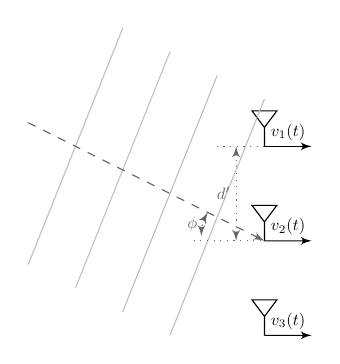
\begin{tikzpicture}[auto, node distance=2cm,>=latex', scale=0.6, every node/.style={scale=0.6}]
        \node [input, name=rxant1] {};
        \node [input, below of=rxant1, node distance=2cm, name=rxant2] {};
        \node [input, below of=rxant2, node distance=2cm, name=rxant3] {};
        \draw [draw] (rxant1) \antenna;
        \draw [draw] (rxant2) \antenna;
        \draw [draw] (rxant3) \antenna;
        \node [input, right of=rxant1, name=output1] {};
        \node [input, right of=rxant2, name=output2] {};
        \node [input, right of=rxant3, name=output3] {};
        \draw [draw,->,align=center] (rxant1) -- node {$v_1(t)$} (output1);
        \draw [draw,->,align=center] (rxant2) -- node {$v_2(t)$} (output2);         
        \draw [draw,->,align=center] (rxant3) -- node {$v_3(t)$} (output3);
        \foreach \x in {0,1,...,3}{
            \draw [draw,-,gray!50] (-0-\x,1+\x/2) -- (-2-\x,-4+\x/2);
        }
        \draw[draw,dashed,->,gray!120] (-5,.5) -- (0,-2);
        \draw[draw,dotted,-,gray!120] (-1.5,-2) -- (0,-2);
        \draw[draw,dotted,<->,gray!120] (-1.2,-1.4) arc (150:180:1) node[midway,anchor=east]{$\phi$};
        \draw[draw,dotted,-,gray!120] (0,0) -- (-1,0);
        \draw[draw,dotted,<->,gray!120] (-.6,0) -- node[anchor=east] {$d'$} (-.6,-2);
        
    \end{tikzpicture}
    \end{figure}
 \end{column}
 \begin{column}{7cm}
    \begin{itemize}
     \item Antennas are very close 
     $$d_i\simeq \overline{d}=\frac{1}{n_r}\sum d_i\forall i$$
     $$|\overrightarrow{P}_1-\overrightarrow{P}_2|\ll \overline{d}\forall i$$
     \item Narrowband $\tau_i-\tau_1\ll T_s \forall i$
     \item $G\simeq e^{-\alpha \overline{d}}$
     \item Simplified received signal
        $v_i(t)=\textcolor{ARust}{e^{-j2\pi \frac{d_i-\overline{d}}{\lambda}}}\sqrt{G}x(t-\overline{\tau})$
     \item Angle of Arrival $\phi$
        $v_i(t)=\textcolor{ARust}{e^{-j2\pi \frac{id'\cos \phi}{\lambda} }}\sqrt{G}x(t-\overline{\tau})$
     \end{itemize}
 \end{column}
\end{columns}
}

\frame{\frametitle{Models For Channel Matrix: Multipath}
    \begin{figure}
     \centering
     \caption{Multipath Channel}
     \includesvg[width=.6\columnwidth]{multipath}
    \end{figure}
    \begin{itemize}
     \item Sum of planar waves with different Ao Departure ($\theta$) and AoA ($\phi$)
     $$h_{i,j}=\sum_{p=1}^{N_{path}}\sqrt{G_p}e^{-j2\pi \frac{d'_i}{\lambda}\cos \theta_p }e^{-j2\pi \frac{d'_j}{\lambda}\cos \phi_p }$$
    \end{itemize}
}


\frame{\frametitle{Models For Channel Matrix: i.i.d. distributions}
\begin{theorem}[Central Limit Theorem]
 For $X_1,X_2,\dots X_n$ samples of an arbitrary probability distribution, $$\lim_{n\to\infty}\sqrt{n}\frac{\frac{1}{n}\sum X_n-\mu}{\sigma}\sim \mathcal{N}(0,1)$$
\end{theorem}

\begin{itemize}
 \item \textbf{Rayleigh fading:} No special paths, $N_{path}\gg n_tn_r$
    $$h_{i,j}\sim\mathcal{CN}(0,\sigma_{z}^2),\;|h_{i,j}|\sim\mathrm{Rayleigh}(\sigma),\;|h_{i,j}|^2\sim\mathrm{Exp}(\frac{1}{\sigma_{z}^2})$$
 \item \textbf{Rice fading:} LOS path $\frac{K}{1+K}$ total power, $N_{path}\gg n_tn_r$
    $$h_{i,j}=\mathcal{CN}(\nu,\sigma_{z}^2),\;K=\frac{\nu^2}{\sigma_{z}^2},\; |h_{i,j}|\sim \mathrm{Rice}(\sigma_{z}^2,K)$$
 \item In MIMO, antennas may or many not be correlated
    $$\textrm{vec}\{\Hb\} \sim \mathcal{CN}(\vv,\K_{\Hb}),\; \textrm{vec}\{\Hb\}\triangleq (h_{1,1},\dots h_{n_r,1},h_{1,2},\dots h_{n_r,n_t})$$
\end{itemize}


}

\frame{\frametitle{Models For SISO Coefficients: i.i.d. distributions}
The following random distributions are common in textbooks for \textbf{single antenna} channels, but they may not be reasonable in MIMO  
\begin{itemize}
 \item \textbf{Nakagami fading:} agrees better than Rayleigh with experimental measurements by Minoru Nakagami in ionospheric short wave
    $$|h|\sim \mathrm{Nakagami}(\sigma_{z}^2,m),|h_{i,j}|^2\sim \mathrm{Gamma}(\frac{1}{\sigma_{z}^2},m)\stackrel{m\in\mathbb{Z}}{=}\mathrm{Erlang}(\frac{1}{\sigma_{z}^2},m)$$
 \item \textbf{2-wave, 3-wave, etc:} only 2, 3, etc. strong paths
    $$\textrm{2-wave}\to h=V_1\times 1+ V_2e^{-j \psi },\; \psi \sim U(0,2\pi)$$
 \item \textbf{Two Wave and Diffuse Propagation:} generalices Rice
    $$h\sim \mathcal{CN}(1+e^{-j \psi },\sigma_{z}^2),\; \psi \sim U(0,2\pi)$$
\end{itemize}
}

% \begin{tikzpicture}

% 
%     \draw (-1,0) -- (5,0);
%     \draw[domain=-0.5:4.5, samples=1000, red] plot (\x, {0.3*sincm(\x*4-3.25)+.5*sincm(\x*4-.75)});
%     \draw (0,1) -- (0,-.1);
%     \draw (1,.1) -- (1,-.1);
%     \draw (2,.1) -- (2,-.1);
%     \draw (3,.1) -- (3,-.1);
%     \draw (4,.1) -- (4,-.1);
% %     \draw[domain=0:0.5, samples=1000, red, dotted] plot (\x,{sinc(\x*20)});
% 
% \end{tikzpicture}

% }

\frame[allowframebreaks]{\frametitle{LOS Beamforming}
\begin{columns}
 \begin{column}{5cm}
    \begin{figure}
    \caption{$\frac{\lambda}{2}$ Uniform Linear Array}
    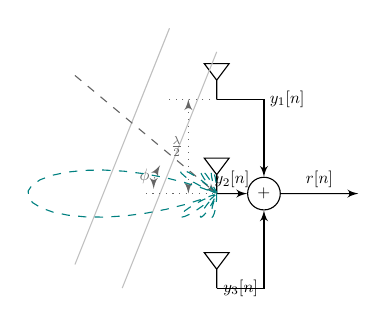
\begin{tikzpicture}[auto, node distance=2cm,>=latex', scale=0.6, every node/.style={scale=0.6}]
        \tikzmath{
        function ULA(\x) {
            if abs(\x) < 0.001 then {
                return 1.0;
            } else {
                return abs(sin(deg(pi*\x/2*8) )/sin(deg(pi/2*\x)))/sqrt(4);
            };
        };
    }

        \node [input, name=rxant1] {};
        \node [input, below of=rxant1, node distance=2cm, name=rxant2] {};
        \node [input, below of=rxant2, node distance=2cm, name=rxant3] {};
        \draw [draw] (rxant1) \antenna;
        \draw [draw] (rxant2) \antenna;
        \draw [draw] (rxant3) \antenna;
        \node [sum, right of=rxant2, name=sum1] {$+$};
        \draw [draw,->,align=center] (rxant1) -| node {$y_1[n]$} (sum1);
        \draw [draw,->,align=center] (rxant2) -- node {$y_2[n]$} (sum1);         
        \draw [draw,->,align=center] (rxant3) -| node {$y_3[n]$} (sum1);
        \node [output, right of=sum1, name=output] {};    
        \draw [draw,->,align=center] (sum1) -- node {$r[n]$} (output);
        \foreach \x in {0,1}{
            \draw [draw,-,gray!50] (-0-\x,1+\x/2) -- (-2-\x,-4+\x/2);
        }
        \draw[draw,dashed,->,gray!120] (-3,.5) -- (0,-2);
        \draw[draw,dotted,-,gray!120] (-1.5,-2) -- (0,-2);
        \draw[draw,dotted,<->,gray!120] (-1.2,-1.4) arc (150:180:1) node[midway,anchor=east]{$\phi$};
        \draw[draw,dotted,-,gray!120] (0,0) -- (-1,0);
        \draw[draw,dotted,<->,gray!120] (-.6,0) -- node[anchor=east] {$\frac{\lambda}{2}$} (-.6,-2);
        \draw[domain=-1:1, samples=100, TZTeal, dashed] plot ({2-ULA(\x)*cos(deg(\x*pi/2))-2}, {ULA(\x)*sin(deg(\x*pi/2))-2});        
    \end{tikzpicture}
    \end{figure}
    $$\y=\h x+\z,\;\h=\left(\begin{array}{c}e^{-j\pi \textcolor{ARust}{0\times}\cos\phi}\\e^{-j\pi \textcolor{ARust}{1\times}\cos\phi}\\\vdots\\e^{-j\pi \textcolor{ARust}{(n_r-1)\times}\cos\phi}\end{array}\right)$$
 \end{column}
 \begin{column}{7cm}
 \begin{itemize}
  \item Array of antennas with sum
  $$r=\sum_{k=1}^{n_r} y_i=\underset{\textnormal{Dirichlett }g(\cos\phi)}{\underbrace{\left(\sum_{k=1}^{n_r} e^{-j\pi k \cos\phi}\right)}}x+z'$$
  \item Equivalent Noise $z'\sim\mathcal{CN}(0,n_r\sigma_{z}^2)$
  \item Equivalent Array Gain $$|g(x)|^2=n_r^2\left|\frac{\sin(\pi n_r x)}{\sin(\pi x)}\right|^2$$
  \item Direction $\phi=0$ SNR$=\frac{\Ex{}{|g(0)x|^2}}{\Ex{}{|z'|^2}}=\frac{n_rP}{\sigma_z^2}$
 \end{itemize}
 \end{column}
\end{columns}


\begin{columns}
 \begin{column}{5cm}
    \begin{figure}
    \caption{Phased-Array Combiner}
    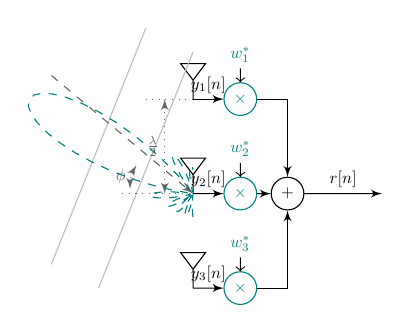
\begin{tikzpicture}[auto, node distance=2cm,>=latex', scale=0.6, every node/.style={scale=0.6}]
        \tikzmath{
        function ULA(\x) {
            if abs(\x) < 0.001 then {
                return 1.0;
            } else {
                return abs(sin(deg(pi*\x/2*8)-30*8 )/sin(deg(pi/2*\x)-30))/sqrt(4);
            };
        };
    }
        \node [input, name=rxant1] {};
        \node [input, below of=rxant1, node distance=2cm, name=rxant2] {};
        \node [input, below of=rxant2, node distance=2cm, name=rxant3] {};
        \draw [draw] (rxant1) \antenna;
        \draw [draw] (rxant2) \antenna;
        \draw [draw] (rxant3) \antenna;        
        \node [sum,color=TZTeal, right of=rxant1, pin={[pinstyle, pin distance=.3cm,color=TZTeal]above:$w_1^*$}] (mult1) {$\times$};
        \node [sum,color=TZTeal, right of=rxant2, pin={[pinstyle, pin distance=.3cm,color=TZTeal]above:$w_2^*$}] (mult2) {$\times$};
        \node [sum,color=TZTeal, right of=rxant3, pin={[pinstyle, pin distance=.3cm,color=TZTeal]above:$w_3^*$}] (mult3) {$\times$};
        \draw [draw,->,align=center] (rxant1) -- node {$y_1[n]$} (mult1);
        \draw [draw,->,align=center] (rxant2) -- node {$y_2[n]$} (mult2);         
        \draw [draw,->,align=center] (rxant3) -- node {$y_3[n]$} (mult3);
        \node [sum, right of=mult2, name=sum1] {$+$};
        \draw [draw,->,align=center] (mult1) -| (sum1);
        \draw [draw,->,align=center] (mult2) -- (sum1);         
        \draw [draw,->,align=center] (mult3) -| (sum1);
        \node [output, right of=sum1, name=output] {};    
        \draw [draw,->,align=center] (sum1) -- node {$r[n]$} (output);
        \foreach \x in {0,1}{
            \draw [draw,-,gray!50] (-0-\x,1+\x/2) -- (-2-\x,-4+\x/2);
        }
        \draw[draw,dashed,->,gray!120] (-3,.5) -- (0,-2);
        \draw[draw,dotted,-,gray!120] (-1.5,-2) -- (0,-2);
        \draw[draw,dotted,<->,gray!120] (-1.2,-1.4) arc (150:180:1) node[midway,anchor=east]{$\phi$};
        \draw[draw,dotted,-,gray!120] (0,0) -- (-1,0);
        \draw[draw,dotted,<->,gray!120] (-.6,0) -- node[anchor=east] {$\frac{\lambda}{2}$} (-.6,-2);
        \draw[domain=-1:1, samples=100, TZTeal, dashed] plot ({2-ULA(\x)*cos(deg(\x*pi/2))-2}, {ULA(\x)*sin(deg(\x*pi/2))-2});        
    \end{tikzpicture}
    \end{figure}
    $$\w(\alpha)=\left(\begin{array}{c}e^{-j\pi 0\times \textcolor{TZTeal}{\alpha}}\\e^{-j\pi 1\times\textcolor{TZTeal}{\alpha}}\\\vdots\\e^{-j\pi (n_r-1)\times\textcolor{TZTeal}{\alpha}}\end{array}\right)$$

 \end{column}
 \begin{column}{7cm}
 \begin{itemize}
  \item Equivalent Channel
    \begin{equation*}
     \begin{split}
        r&=\w(\alpha)^H\y=(\w(\alpha)^H\h) x+z'\\
         &= \left(\sum_{k=1}^{n_r} e^{-j\pi k (\cos(\phi)-\textcolor{TZTeal}{\alpha})}\right)x+z'
     \end{split}
    \end{equation*}
  \item $\alpha$ changes angle of maximum gain
 $$|\w(\phi)^H\h|^2=|g(\cos(\phi)-\textcolor{TZTeal}{\alpha}))|^2$$
 \item Optimum 
 $$\alpha^*=\cos\phi\to|\w^H\h|^2=n_r^2\to\textnormal{SNR}=\frac{n_rP}{\sigma_z^2}$$
 \item \textbf{Electronically Steerable Antenna / Smart Antenna}
 \end{itemize}
 \end{column}
\end{columns}
}


\frame[allowframebreaks]{\frametitle{Algebraic Beamforming}

\begin{figure}
 \centering
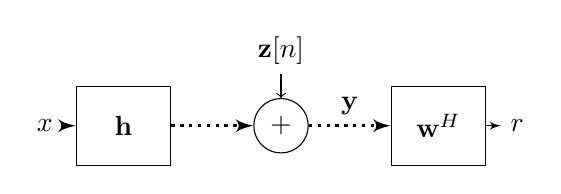
\begin{tikzpicture}[auto, node distance=2cm,>=latex']
    \node [pinstyle] (tx) {$x$};
    \node [block,right of=tx, node distance=1cm] (mult) {$\h$};
    \draw [->,dotted,very thick] (tx) -- (mult);
    \node [sum, right of=mult, node distance=2cm, pin={[pinstyle, pin distance=.3cm]above:$\z[n]$}] (sum) {$+$};
    \draw [->,dotted,very thick] (mult) -- (sum);
     \node [block,right of=sum] (mult2) {$\w^H$};
    \draw [->,dotted,very thick] (sum) -- node{$\y$} (mult2);
    \node [pinstyle, right of=mult2, node distance=1cm] (rec) {$r$};
    \draw [->] (mult2) -- (rec);
\end{tikzpicture}
 \caption{ AWGN SIMO DEC combining} 
\end{figure}
 \begin{itemize}
  \item Linear combination with $\y=\h x + \z$
  $$r=\w^H\y= \w^H\h x + \cancel{\w^H\z}^{z'}$$
  \item Maximize SNR $\max \frac{\Ex{}{|\w^H\h x|^2}}{\Ex{}{|z'|^2}}=\max \frac{\Ex{}{|\w^H\h|^2}}{\Ex{}{\|\w\|^2}}\frac{P}{\sigma_{z}^2}$
  \item Noise power grows with $\Ex{}{\|\w\|^2}\to$ unitary vector\\ \ \\
  
  \item \textbf{Maximal Ratio Combining} $\w^H=\frac{\h^H}{\|\h\|}\to$ SNR$=\|\h\|^2\frac{P}{\sigma_{z}^2}=\frac{n_rP}{\sigma_{z}^2}$
 \end{itemize}
\begin{columns}
 \begin{column}{6cm}
    \begin{figure}
    \caption{Project $\y$ to subspace base $\h$ }
     \includesvg[width=.6\columnwidth]{projection1}
    \end{figure}
    \vspace{.5cm}
 \end{column}
 \begin{column}{6cm}
    \begin{figure}
    \caption{No physical direction}
     \includesvg[width=.6\columnwidth]{csihbf}
    \end{figure}
 \end{column}
\end{columns}
    \textbf{\textcolor{ARust}{DIGITAL MIMO SURPASSES SMART ANTENNA ARRAYS}}
}
\end{document}


